\documentclass[article,12pt]{elsarticle}
\usepackage[utf8]{inputenc}
\usepackage{graphicx}
\usepackage{booktabs}
\usepackage{subcaption}
\usepackage{amssymb}
\usepackage{flushend}
\usepackage{float}
\usepackage{amsmath}
\usepackage{amsfonts}
\usepackage{dcolumn}
\usepackage{amsthm}
\usepackage{caption}
\usepackage{lmodern}
\usepackage{booktabs}
\usepackage{color}
\usepackage{longtable}
\usepackage{rotating}
\usepackage{etoolbox}
\usepackage{hyperref}
\usepackage{comment}
\usepackage{pdflscape}
\usepackage{comment}
\usepackage[table,xcdraw]{xcolor}
\usepackage[framemethod=TikZ]{mdframed}
\newcommand{\aw}{\textcolor{purple}{\textit{answer}:\quad}}

\begin{document}

%1. Exprese \( D \subset \mathbb{R}^{2} \) como una región Tipo I y Tipo II. Después resuelva las dos integrales, esto es, en la región Tipo I y en la región Tipo II. Finalmente dibuje las regiones de integración. \\
a) \( \iint_{D} x d A \) donde \( D \) esta encerrada por las rectas \( y=x, y=0 \) y \( x=1 \).
Para una región Tipo I, la región D se describe como \( D = \{ (x, y) \mid a \leq x \leq b, g_{1}(x) \leq y \leq g_{2}(x) \} \).

\( x \) varía desde \( 0 \) hasta \( 1 \) (por las rectas \( y = x \) y \( x = 1 \)). \\
\( y \) varía desde \( 0 \) hasta \( x \) (por las rectas \( y = 0 \) y \( y = x \)). \\

Entonces, la región Tipo I es:
\[
D = \{(x, y) \mid 0 \leq x \leq 1, 0 \leq y \leq x\}
\]
La integral es:
\[
\iint_{D} x \, dA = \int_{0}^{1} \int_{0}^{x} x \, dy \, dx
\]
Separamos la integral doble en un producto de dos integrales (recordemos que esto es aplicable cuando tienes una función integrada respecto de $x$ y $y$ $f(x,y)=g(x)h(y)$). En tanto y se tiene,
\[
   \int_{0}^{x} x \, dy = x \cdot y \bigg|_{0}^{x} = x^2
   \]

Ahora con respecto a x:
\[
   \int_{0}^{1} x^2 \, dx = \left[\frac{x^3}{3}\right]_{0}^{1} = \frac{1}{3}
   \]

Por otra parte para una región Tipo II, la región D se describe como \( D = \{ (x, y) \mid c \leq y \leq d, h_{1}(y) \leq x \leq h_{2}(y) \} \). Aquí \( y \) varía desde \( 0 \) hasta \( 1 \) en tanto $x$ varía desde $y$ hasta 1.

Entonces, la región Tipo II es:
\[
D = \{(x, y) \mid 0 \leq y \leq 1, y \leq x \leq 1\}
\]

La integral para esta región es:
\[
\iint_{D} x \, dA = \int_{0}^{1} \int_{y}^{1} x \, dx \, dy
\]

Usamos la misma propiedad de separar como un producto de integrales. Veamos que para $x$:
\[
   \int_{y}^{1} x \, dx = \left[\frac{x^2}{2}\right]_{y}^{1} = \frac{1}{2} - \frac{y^2}{2}
   \]
Con respecto a $y$ se tiene.
\[
   \int_{0}^{1} \left(\frac{1}{2} - \frac{y^2}{2}\right) \, dy = \left[ \frac{y}{2} - \frac{y^3}{6} \right]_{0}^{1} = \frac{1}{2} - \frac{1}{6} = \frac{1}{3}
   \]

\begin{figure}[h]
    \centering
    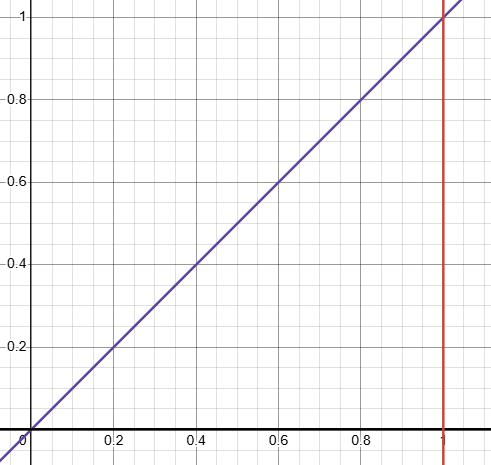
\includegraphics[width=0.5\linewidth]{1a.png}
    \caption{Región de integración a)}
    \label{fig:enter-label}
\end{figure}

b) \( \iint_{D}|x y| d A \) donde \( D \) esta encerrada por las curvas \( y=x^{2} \) y \( y=3 x \). \\

Para expresar D como una región Tipo I y Tipo II, primero identificamos las curvas $y=x^2$ y $y=3x$, que se intersectan en $x=0$ y $x=3$ ($x^2 - 3x = 0 \implies x(x - 3) = 0$).
Región Tipo I: \( D \) es el conjunto de puntos \((x, y)\) tal que \( 0 \leq x \leq 3 \) y \( x^2 \leq y \leq 3x \). La integral se describe como sigue.
\[
\int_{0}^{3} \int_{x^2}^{3x} |xy| \, dy \, dx
\]
Región Tipo II: D es el conjunto de puntos (x,y) tal que \( 0 \leq y \leq 9 \) y \( \sqrt{y} \leq x \leq \frac{y}{3} \). La integral es:
\[
\int_{0}^{9} \int_{\sqrt{y}}^{y/3} |xy| \, dx \, dy
\]
Ahora, resolveremos ambas integrales; para la integral Tipo I:
\[
\int_{0}^{3} \int_{x^2}^{3x} |xy| \, dy \, dx = \int_{0}^{3} \int_{x^2}^{3x} xy \, dy \, dx = \int_{0}^{3} \left[\frac{xy^2}{2}\right]_{y=x^2}^{y=3x} \, dx = \int_{0}^{3} \left(\frac{9x^3}{2} - \frac{x^5}{2}\right) \, dx
\]
\[
= \int_{0}^{3} \frac{9x^3 - x^5}{2} \, dx = \frac{1}{2} \left[\frac{9x^4}{4} - \frac{x^6}{6}\right]_{0}^{3} = \frac{1}{2} \left(\frac{9 \times 81}{4} - \frac{729}{6}\right) = 30.375
\]
Para la integral Tipo II:
\[
\int_{0}^{9} \int_{\sqrt{y}}^{y/3} |xy| \, dx \, dy = \int_{0}^{9} \int_{\sqrt{y}}^{y/3} xy \, dx \, dy = \int_{0}^{9} \left[\frac{x^2y}{2}\right]_{x=\sqrt{y}}^{x=y/3} \, dy = \int_{0}^{9} \left(\frac{y^3}{18} - \frac{y^2\sqrt{y}}{2}\right) \, dy
\]
\[
= \int_{0}^{9} \left(\frac{y^3}{18} - \frac{y^{5/2}}{2}\right) \, dy = \left[\frac{y^4}{72} - \frac{y^{7/2}}{7}\right]_{0}^{9} = \left(\frac{9^4}{72} - \frac{9^{7/2}}{7}\right) = 30.375
\]

\begin{figure}[h]
    \centering
    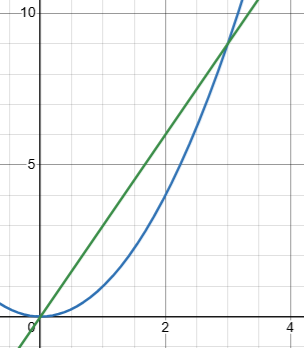
\includegraphics[width=0.5\linewidth]{1b.png}
    \caption{Región de integración b)}
    \label{fig:enter-label}
\end{figure}
%2. Plantee las siguientes integrales dobles en ambos órdenes de integración. Después resuelva la integral usando el orden más sencillo (SÓLO resuelva uno).\\
a) \( \iint_{D} y d A \) donde \( D \subset \mathbb{R}^{2} \) está acotada por \( y=x-2 \) y \( x=y^{2} \). \\
La región \( D \) está delimitada por \( y = x - 2 \) y \( x = y^2 \). Esto nos da los siguientes despejes bastante simples:
\begin{itemize}
    \item Región tipo I: \( 2 \leq x \leq 3 \), \( \sqrt{x} \leq y \leq x - 2 \).  
    \item Región tipo II: \( 0 \leq y \leq 1 \), \( y^2 \leq x \leq y + 2 \).  
\end{itemize}

Ambas parecen casi igual de difíciles, pero en general las raíces a veces son complicadas de interpretar así que resolvemos en Tipo II:  

\[
I = \int_0^1 \int_{y^2}^{y+2} y \, dx \, dy = \int_0^1 y (y + 2 - y^2) dy = \int_0^1 (y^2 + 2y - y^3) dy = \left( \frac{1}{3} + 1 - \frac{1}{4} \right) = \frac{13}{12}.
\]

b) \( \iint_{D} y^{2} e^{x y} d A \) donde \( D \subset \mathbb{R}^{2} \) está acotada por \( y=x, y=4 \) y \( x=0 \). \\
La región \( D \) está acotada por \( y = x \), \( y = 4 \) y \( x = 0 \). Este es más sencillo que el anterior pues tenemos y=x así que solo cambia una pequeña parte.
\begin{itemize}
    \item Región tipo I: \( 0 \leq x \leq 4 \), \( x \leq y \leq 4 \).  
    \item Región tipo II: \( 0 \leq y \leq 4 \), \( 0 \leq x \leq y \).  
\end{itemize}

Resolvemos en Tipo II:  

\[
I = \int_0^4 \int_0^y y^2 e^{xy} \, dx \, dy = \int_0^4 y^2 \left[ \frac{e^{xy}}{y} \Big|_0^y \right] dy = \int_0^4 y^2 \frac{e^{y^2} - 1}{y} dy = \int_0^4 (y e^{y^2} - y) dy
\]
\[
= \frac{1}{2} \int_0^{16} e^u du - \int_0^4 y dy. = \frac{e^{16} - 1}{2} - 8.
\]  

c) \( \iint_{D} \operatorname{sen}(x) d A \) donde \( D=\left\{(x, y) \in \mathbb{R}^{2} ; \frac{-\pi}{2} \leq y \leq \frac{\pi}{2},-y-\frac{\pi}{2} \leq x \leq y\right\} \). \\

La región \( D \) está definida por \( -\frac{\pi}{2} \leq y \leq \frac{\pi}{2} \) y \( -y - \frac{\pi}{2} \leq x \leq y \). De aquí nótese que tenemos.
\begin{itemize}
    \item Región tipo I: \( -\frac{\pi}{2} \leq x \leq \frac{\pi}{2} \), \( -x - \frac{\pi}{2} \leq y \leq x \).  
    \item Región tipo II: \( -\frac{\pi}{2} \leq y \leq \frac{\pi}{2} \), \( -y - \frac{\pi}{2} \leq x \leq y \).  
\end{itemize}

Resolvemos en Tipo II:  

\[
I = \int_{-\frac{\pi}{2}}^{\frac{\pi}{2}} \int_{-y - \frac{\pi}{2}}^y \sin(x) \, dx \, dy.
\]

Resolvemos primero la integral interna que es bastante simple,

\[
\int \sin(x) dx = -\cos(x).
\]

Evaluamos en los límites

\[
-\cos(y) + \cos(-y - \frac{\pi}{2}).
\]

Como \( \cos(-y - \frac{\pi}{2}) = \sin(y) \), tenemos:

\[
I = \int_{-\frac{\pi}{2}}^{\frac{\pi}{2}} (-\cos(y) + \sin(y)) dy = -\int_{-\frac{\pi}{2}}^{\frac{\pi}{2}} \cos(y) dy + \int_{-\frac{\pi}{2}}^{\frac{\pi}{2}} \sin(y) dy -\sin(y) \Big|_{-\frac{\pi}{2}}^{\frac{\pi}{2}} + (-\cos(y)) \Big|_{-\frac{\pi}{2}}^{\frac{\pi}{2}} 
\]
\[
= - (1 - (-1)) + (-0 + 0) = - (1 + 1) + 0 = -2 = -2
\]

d) \( \iint_{D} \frac{y}{x^{5}+1} d A \) donde \( D=\left\{(x, y) \in \mathbb{R}^{2} ; 0 \leq x \leq 1,0 \leq y \leq x^{2}\right\} \). \\
La región \( D \) está dada por \( 0 \leq x \leq 1 \), \( 0 \leq y \leq x^2 \). Se sigue que.
\begin{itemize}
    \item Región tipo I: \( 0 \leq x \leq 1 \), \( 0 \leq y \leq x^2 \).  
    \item Región tipo II: \( 0 \leq y \leq 1 \), \( 0 \leq x \leq \sqrt{y} \).  

Resolvemos en Tipo I:  

\[
I = \int_0^1 \int_0^{x^2} \frac{y}{x^5+1} dy \, dx.
\]

Hacemos la integral interna como de costumbre:

\[
\int_0^{x^2} \frac{y}{x^5+1} dy = \frac{1}{x^5+1} \int_0^{x^2} y dy = \frac{1}{x^5+1} \cdot \frac{y^2}{2} \Big|_0^{x^2} = \frac{x^4}{2(x^5+1)}.
\]

Ahora la integral externa:

\[
I = \int_0^1 \frac{x^4}{2(x^5+1)} dx.
\]

Es demasiado sugerente el logaritmo natural como primitiva de la función integrada, pero lo haremos más visible con el cambio \( u = x^5 + 1 \), con \( du = 5x^4 dx \), veamos que entonces:

\[
I = \frac{1}{10} \int_1^2 \frac{du}{u} = \frac{1}{10} \ln |u| \Big|_1^2 = \frac{1}{10} (\ln 2 - \ln 1) = \frac{\ln 2}{10}.
\]
3. Resuelva las siguientes integrales dobles usando el orden de integración que prefiera y dibuje las regiones de integración así como las superficies \( z=f(x, y) \). \\
a) \( \iint_{D} x \cos (y) d A \) donde \( D \subset \mathbb{R}^{2} \) está acotada por \( y=0, y=x^{2} \) y \( x=1 \). \\
La región \( D \) está delimitada por \( y = 0 \), \( y = x^2 \) y \( x = 1 \), lo que implica que como región I es \( 0 \leq x \leq 1 \), \( 0 \leq y \leq x^2 \).  

\[
I = \int_0^1 \int_0^{x^2} x \cos(y) \, dy \, dx.
\]

La integral interna:

\[
\int_0^{x^2} x \cos(y) \, dy = x \sin(y) \Big|_0^{x^2} = x \sin(x^2).
\]

La integral externa:

\[
I = \int_0^1 x \sin(x^2) dx.
\]

Hacemos \( u = x^2 \), entonces \( du = 2x dx \):

\[
I = \frac{1}{2} \int_0^1 \sin u \, du = \frac{1}{2} (-\cos u) \Big|_0^1 = \frac{1}{2} (-\cos 1 + 1)  = \frac{1 - \cos 1}{2}.
\]
b) \( \iint_{D}\left(x^{2}+2 y\right) d A \) donde \( D \subset \mathbb{R}^{2} \) está acotada por \( y=x, y=x^{3} \) y \( x \geq 0 \). \\
c) \( \iint_{D} \ln (y) d A \) donde \( D \subset \mathbb{R}^{2} \) es la región triángular con vértices en: \( (0,1),(1,2),(4,1) \). \\
d) \( \iint_{D} x y^{2} d A \) donde \( D \subset \mathbb{R}^{2} \) es la región encerrada por \( x=0 \) y \( x=\sqrt{1-y^{2}} \). \\
%5. Al evaluar una integral doble sobre una región \( D \) se obtuvo una suma de integrales iteradas como sigue:
\[
\iint_{D} f(x, y) d A=\int_{0}^{1} \int_{0}^{2 y} f(x, y) d x d y+\int_{1}^{3} \int_{0}^{3-y} f(x, y) d x d y
\]

Describa la región \( D \) y exprese la integral doble como una integral iterada con el OTRO orden de integración. Finalmente dibuje la región \( D \). \\

Analicemos los límites de integración en cada término:  

Para la primera integral reunimos las siguientes características.
\begin{itemize}
    \item \( y \) varía de \( 0 \) a \( 1 \).
   \item Para cada \( y \), \( x \) varía de \( 0 \) a \( 2y \).
\end{itemize}

Para la segunda.
\begin{itemize}
    \item \( y \) varía de \( 1 \) a \( 3 \).
   \item Para cada \( y \), \( x \) varía de \( 0 \) a \( 3 - y \).
\end{itemize}

Combinando ambas partes, la región \( D \) es:

\[
D = \{(x,y) \in \mathbb{R}^2 \mid 0 \leq x \leq 3, 0 \leq y \leq g(x)\},
\]

donde \( g(x) \) es la frontera superior de \( y \) en términos de \( x \); vease que para \( 0 \leq x \leq 2 \), despejamos \( y \) de \( x \leq 2y \):  
  \[
  y \geq \frac{x}{2}.
  \]
  Ahora para \( 2 \leq x \leq 3 \), despejamos \( y \) de \( x \leq 3 - y \):  
  \[
  y \leq 3 - x.
  \]

Por lo tanto, la región \( D \) está acotada por \( x \) en \( [0,3] \), y por \( y \) en:

\[
\frac{x}{2} \leq y \leq 3 - x.
\]

El orden actual es \( dy \) externo y \( dx \) interno. Para cambiar el orden, describimos \( D \) en términos de \( x \) como variable externa, obsérvese que \( x \) varía entre \( 0 \) y \( 3 \), además para cada \( x \), \( y \) varía entre \( \frac{x}{2} \) y \( 3 - x \). \\

La nueva integral es:

\[
\iint_D f(x,y) dA = \int_0^3 \int_{\frac{x}{2}}^{3-x} f(x,y) \,dy\,dx.
\]

Miremos que la recta \( x = 2y \) pasa por \( (0,0) \) y \( (2,1) \); la recta \( x = 3 - y \) pasa por \( (3,0) \) y \( (0,3) \); la región está delimitada por estas curvas en \( 0 \leq x \leq 3 \). Esto nos denota 3 intersecciones expresadas como un triángulo con vértices en \( (0,0) \), \( (2,1) \) y \( (3,0) \).

\begin{figure}[h]
    \centering
    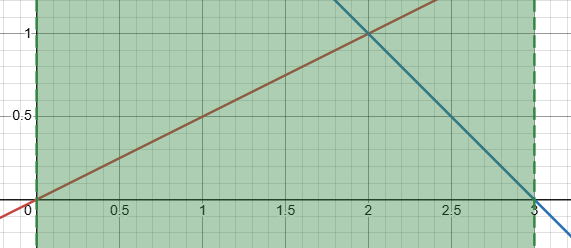
\includegraphics[width=0.5\linewidth]{triangle5.png}
    \caption{Región descrita en el Ejercicio V}
    \label{fig:enter-label}
\end{figure}
%6. Use el Teorema de Cambio de Variable en los siguientes incisos. \\
a) Sea \( T: \mathbb{R}^{2} \rightarrow \mathbb{R}^{2} \) la transformación definida por \( T(u, v)=(4 u, 2 u+3 v) \) y sea \( D^{*}=[0,1] \times[1,2] \). Encuentre \( D \subset \mathbb{R}^{2} \) tal que \( D=T\left(D^{*}\right) \) y resuelva \( \iint_{D}(x-y) d x d y \). \\
Para encontrar D, transformamos los límites de u y v en distintas fases...\\
Cuando u=0 y v varía de 1 a 2:
\[
  (x, y) = T(0, v) = (0, 3v) \implies (x=0, y \in [3, 6])
  \]


Cuando u=1 y v varía de 1 a 2:
\[
  (x, y) = T(1, v) = (4, 2 + 3v) \implies (x=4, y \in [5, 8])
  \]


Cuando v=1 y u varía de 0 a 1:
\[
  (x, y) = T(u, 1) = (4u, 2u + 3) \implies (x \in [0, 4], y = 2u + 3)
  \]


Cuando v=2 y u varía de 0 a 1:
\[
  (x, y) = T(u, 2) = (4u, 2u + 6) \implies (x \in [0, 4], y = 2u + 6)
  \]


Por lo tanto, se descubrió que la región D es un paralelogramo con vértices en (0,3), (0,6), (4,5), y (4,8); calcúlese ahora el jacobiano de T.

\[
J = \begin{vmatrix}
\frac{\partial x}{\partial u} & \frac{\partial x}{\partial v} \\
\frac{\partial y}{\partial u} & \frac{\partial y}{\partial v}
\end{vmatrix}
= \begin{vmatrix}
4 & 0 \\
2 & 3
\end{vmatrix}
= 4 \cdot 3 - 0 \cdot 2 = 12
\]

La integral queda como sigue,
\[
\iint_{D^*} (4u - (2u + 3v)) \cdot 12 \, du \, dv = \iint_{D^*} (2u - 3v) \cdot 12 \, du \, dv = 12 \int_{0}^{1} \int_{1}^{2} (2u - 3v) \, dv \, du
\]

Primero resolvemos la integral interna respecto a v: \\
\begin{align*}
\int_{1}^{2} (2u - 3v) \, dv &= \left[ 2uv - \frac{3v^2}{2} \right]_{v=1}^{v=2} \\
&= \left(2u \cdot 2 - \frac{3 \cdot 2^2}{2}\right) - \left(2u \cdot 1 - \frac{3 \cdot 1^2}{2}\right) \\
&= \left(4u - 6\right) - \left(2u - \frac{3}{2}\right) \\
&= 4u - 6 - 2u + \frac{3}{2} \\
&= 2u - \frac{9}{2}
\end{align*}

Finalmente respecto a u:
\begin{align*}
12 \int_{0}^{1} \left(2u - \frac{9}{2}\right) \, du
&= 12 \left[ u^2 - \frac{9}{2}u \right]_{0}^{1}  \\
&= 12 \left(1^2 - \frac{9}{2} \cdot 1\right) - 12 \left(0^2 - \frac{9}{2} \cdot 0\right)  \\
&= 12 \left(1 - \frac{9}{2}\right) \\
&= 12 \left(\frac{2}{2} - \frac{9}{2}\right) \\
&= 12 \left(-\frac{7}{2}\right) \\
&= -42 
\end{align*}

b) Calcule la integral \( \iint_{R}(x-y)^{2} \operatorname{sen}^{2}(x+y) d x d y \); donde \( R \) es el paralelogramo de vértices \( (0, \pi) \), \( (\pi, 0),(2 \pi, \pi) \) y \( (\pi, 2 \pi) \). \\

Dado el paralelogramo con vértices $(0,\pi), (\pi,0), (2\pi,\pi),\text{ y }(\pi,2\pi)$, utilizamos una transformación lineal para simplificar el cálculo; usamos $T(u,v)=(u+v,u−v)$. Nótese que.
\begin{itemize}
    \item Esta transformación mapea $(0,\pi)\textit{ a }(0,0)$
    \item Mapea $(\pi,0)\text{ a }(\pi,0)$
    \item Mapea $(2\pi,\pi)\text{ a }(2\pi,0)$
    \item Mapea $(\pi,2\pi)\text{ a }(\pi,−\pi)$
\end{itemize}

Calculamos el jacobiano de T que es simplemente el determinante de la siguiente matriz.
\[
   J = \left| \begin{matrix} 
   1 & 1 \\ 
   1 & -1 
   \end{matrix} \right| = -2
   \]

La integral entonces es:
\[
   \iint_{R} (x-y)^2 \sin^2(x+y) \, dx \, dy = \iint_{R'} (2v)^2 \sin^2(2u) \cdot (-2) \, du \, dv
   \]

Veamos que $u$ varía de $0 \rightarrow 2\pi$, $v$ varía de $0 \rightarrow \pi$, se sigue que.
\[
   = -8 \int_{0}^{2\pi} \int_{0}^{\pi} v^2 \sin^2(2u) \, dv \, du
   \]

De aquí puede observarse que la integral se puede calcular por separado con respecto a $u$ y $v$. Por un lado

\[
     \int_{0}^{\pi} v^2 \, dv = \left[ \frac{v^3}{3} \right]_{0}^{\pi} = \frac{\pi^3}{3}, \text{por el otro...}
     \]

\[
     -8 \cdot \frac{\pi^3}{3} \int_{0}^{2\pi} \sin^2(2u) \, du
     \]


Usamos la identidad \(\sin^2(\theta) = \frac{1 - \cos(2\theta)}{2}\):
\[
     \int_{0}^{2\pi} \sin^2(2u) \, du = \int_{0}^{2\pi} \frac{1 - \cos(4u)}{2} \, du = \pi
     \]

Finalmente al multiplicar estas dos integrales obtenemos lo siguiente.
\[
   -8 \cdot \frac{\pi^3}{3} \cdot \pi = -\frac{8\pi^4}{3}
   \]

c) Sea \( D=\left\{(x, y) \in \mathbb{R}^{2} \mid x^{2}+y^{2} \leq 4\right\} \). Resuelva \( \iint_{D} e^{\left(x^{2}+y^{2}\right)} d x d y \). \\

Para esta integral, es conveniente usar coordenadas polares porque la región D es un disco. Consideramos la transformación a coordenadas polares ($x=rcos\theta, \qquad y=rsin\theta, \qquad r^2 = x^2+y^2, \qquad dxdy=rdrd\theta$). Establezcamos los límites de integración, por la desigualdad presentada se sabe que $r$ varía de 0 a 2, el ángulo en tanto al ser un disco varía de 0 a $2\pi$.

\[
   \iint_{D} e^{x^2 + y^2} \, dx \, dy = \int_{0}^{2\pi} \int_{0}^{2} e^{r^2} \cdot r \, dr \, d\theta
   \]

Usamos la misma técnica de separar la integral doble en un producto de integrales pues la función se separa en una parte términos de $u$ y otra parte en términos de $v$. Primero resolvemos para $u$.

\[
     \frac{1}{2} \int_{0}^{4} e^u \, du = \frac{1}{2} \left[ e^u \right]_{0}^{4} = \frac{1}{2} (e^4 - e^0) = \frac{1}{2} (e^4 - 1)
     \]

Véase que aunque parezca que la función en términos de $\theta$ es cero en realidad es $1\circ\theta=1$.
\[
     \int_{0}^{2\pi} d\theta = 2\pi
     \]
Multiplicando tenemos el resultado final.
\[
   2\pi \cdot \frac{1}{2} (e^4 - 1) = \pi (e^4 - 1)
   \]

d) Use la transformación \( T(u, v)=(u-u v, u v) \) para calcular \( \iint_{R} \frac{1}{x+y} d x d y \) donde \( R \) es la región acotada por los planos \( x=0, y=0, x+y=1 \) y \( x+y=4 \). \\

La región está acotada por los planos $x=0, y=0, x+y=1, \text{ y  } x+y=4$. Calculamos el determinante del jacobiano de T:
\[
   J = \begin{vmatrix}
   \frac{\partial x}{\partial u} & \frac{\partial x}{\partial v} \\
   \frac{\partial y}{\partial u} & \frac{\partial y}{\partial v}
   \end{vmatrix}
   = \begin{vmatrix}
   1 - v & -u \\
   v & u
   \end{vmatrix}
   = u(1-v) + uv = u
   \]


Notemos que los límites de integración varían para $u$ de $1 \rightarrow 4$ (determinado por x+y=1 y x+y=4). Por otro lado $v$ varía de $0 \rightarrow 1$ (ya que $y=uv$ y $y$ varía de $0 \rightarrow u$). \\

La integral transformada es.
\[
   \iint_{R} \frac{1}{x+y} \, dx \, dy = \iint_{R'} \frac{1}{u} \cdot u \, dv \, du = \int_{1}^{4} \int_{0}^{1} 1 \, dv \, du
   \]

Separamos la integral nuevamente; respecto a $v$,
\[
     \int_{0}^{1} 1 \, dv = [v]_{0}^{1} = 1
     \]

Respecto a $u$.
\[
     \int_{1}^{4} 1 \, du = [u]_{1}^{4} = 4 - 1 = 3
     \]

La multiplicación es simplemente 3 que es el resultado final.\\\\
%8. Considere el elipsoide \( E=\left\{(x, y, z) \in \mathbb{R}^{3} \left\lvert\, \frac{x^{2}}{a^{2}}+\frac{y^{2}}{b^{2}}+\frac{z^{2}}{c^{2}} \leq 1\right.\right\} \), con \( a, b \) y \( c \) números reales positivos. \\
a) Calcule el volúmen de \( E \). \\
\aw Usamos el cambio de coordenadas esféricas con una sutileza en el coeficiente de cada variable.
\begin{align*}
    x &= a\rho sin\phi cos\theta \\
y &= b\rho sin\phi sin\theta \\
z &= c\rho cos\phi
\end{align*}

Donde $\rho, \phi \text{  y  } \theta$ son las coordenadas esféricas. Dado que trabajamos con una elipsoide nos gustaría trabajar con un problema que ya conocemos, las coordenadas esféricas, para ello necesitamos que sea una "esfera" que crece a diferentes velocidades para radios de cero a uno en las distintas 3 coordenadas, definimos el radio $\rho$ que llegue hasta uno pero dadas las condiciones en cada coordenada, en x se extenderá hasta un "radio a" (entre comillas porque la noción de radio está degenerada, es más bien un eje), en y radio b y en z radio c; por lo que nuestros parámetros se limitan como sigue:
\begin{itemize}
    \item $\rho$ varía de 0 a 1
    \item $\phi$ varía de 0 a $\pi$
    \item $\theta$ varía de 0 a 2$\pi$
\end{itemize}

El jacobiano de esta transformación es muy similar al de coordenadas esféricas "ordinarias", por propiedades de los determinantes podemos "factorizar" el término de una fila extrayéndolo del determinante. Al hacer esto tenemos el jacobiano de la transformación esférica que ya conocemos:
\[
J = \begin{vmatrix}
a \sin \phi \cos \theta & a \rho \cos \phi \cos \theta & -a \rho \sin \phi \sin \theta \\
b \sin \phi \sin \theta & b \rho \cos \phi \sin \theta & b \rho \sin \phi \cos \theta \\
c \cos \phi & -c \rho \sin \phi & 0
\end{vmatrix} = 
abc\begin{vmatrix}
\sin \phi \cos \theta & \rho \cos \phi \cos \theta & - \rho \sin \phi \sin \theta \\
\sin \phi \sin \theta & \rho \cos \phi \sin \theta & \rho \sin \phi \cos \theta \\
\cos \phi & -\rho \sin \phi & 0
\end{vmatrix} 
\]
\[
J =
abc \rho^2 \sin \phi
\]
Por lo tanto, el volumen del elipsoide es:
\[
V = \int_{0}^{2\pi} \int_{0}^{\pi} \int_{0}^{1} abc \rho^2 \sin \phi \, d\rho \, d\phi \, d\theta
\]
Resolvemos la integral separándola en 3, usando el mismo argumento de incisos anteriores pero generalizado para funciones de la forma $f(x,y,z)=f_1(x)f_2(y)f_3(z)$.\\

Integral respecto a $\rho$:
\[
  \int_{0}^{1} \rho^2 \, d\rho = \left[ \frac{\rho^3}{3} \right]_{0}^{1} = \frac{1}{3}
  \]


Integral respecto a $\phi$:
\[
  \int_{0}^{\pi} \sin \phi \, d\phi = \left[ -\cos \phi \right]_{0}^{\pi} = 2
  \]


Integral respecto a $\theta$:
\[
  \int_{0}^{2\pi} \, d\theta = 2\pi
  \]


Por lo tanto, el volumen es:
\[
V = abc \cdot \frac{1}{3} \cdot 2 \cdot 2\pi = \frac{4}{3} \pi abc
\]

b) Resuelva \( \iiint_{E}|x y z| d x d y d z \). \\
\aw Usamos la misma transformación:
\[
\iiint_{E} |x y z| \, dx \, dy \, dz = \int_{0}^{2\pi} \int_{0}^{\pi} \int_{0}^{1} |a b c \rho^3 \sin^2 \phi \cos \theta \sin \theta \cos \phi| \cdot abc \rho^2 \sin \phi \, d\rho \, d\phi \, d\theta
\]
Simplificamos la integral:
\[
= a^2 b^2 c^2 \int_{0}^{2\pi} \int_{0}^{\pi} \int_{0}^{1} \rho^5 \sin^3 \phi |\cos \theta \sin \theta \cos \phi| \, d\rho \, d\phi \, d\theta
\]

Separamos nuevamente; integral respecto a $\rho$:
\[
   \int_{0}^{1} \rho^5 \, d\rho = \left[ \frac{\rho^6}{6} \right]_{0}^{1} = \frac{1}{6}
   \]


Integral respecto a $\phi$:
\[
   \int_{0}^{\pi} \sin^3 \phi |\cos \phi| \, d\phi
   \]

Dividimos en dos partes, de \(0\) a \(\frac{\pi}{2}\) y de \(\frac{\pi}{2}\) a \(\pi\), ya que \(|\cos \phi|\) cambia de signo.

\[
   = 2 \int_{0}^{\frac{\pi}{2}} \sin^3 \phi \cos \phi \, d\phi = 2 \cdot \frac{1}{4} = \frac{1}{2}
   \]


Integral respecto a $\theta$:
\[
   \int_{0}^{2\pi} |\cos \theta \sin \theta| \, d\theta = \int_{0}^{2\pi} \frac{1}{2} |\sin(2\theta)| \, d\theta
   \]

Evaluamos desde 0 a $\pi$, multiplicamos por 2 por simetría:
\[
   = 2 \cdot \int_{0}^{\pi} \frac{1}{2} \sin(2\theta) \, d\theta = 2 \cdot \left[-\frac{1}{4} \cos(2\theta)\right]_{0}^{\pi} = 2 \cdot \frac{1}{2} = 1
   \]



Por lo tanto, el resultado de la integral es:
\[
a^2 b^2 c^2 \cdot \frac{1}{6} \cdot \frac{1}{2} \cdot 1 = \frac{a^2 b^2 c^2}{12}
\]


\end{document}
